\documentclass[12pt]{book}
\title{Física y Química Adaptada para ESO}
\author{José Ignacio Otero Bueno}
\usepackage[spanish]{babel}
\usepackage[utf8]{inputenc}
\usepackage{amssymb, amsmath, amsbsy}
\usepackage{schemata} 
\usepackage{stackrel}
\usepackage{multicol}
\usepackage{fullpage}
\usepackage{textcomp}
\usepackage{cite}
\usepackage{graphicx}
\usepackage[		
top=2.5cm,			% Margen superior
bottom=2.5cm,		% Margen inferior
inner=2.5cm,		% Margen al interior
outer=2.5cm			% Margen al exterior
]{geometry}
\usepackage[usenames,dvipsnames,svgnames,table]{xcolor}
\usepackage{afterpage}
\usepackage{setspace}
\usepackage{hyperref}


%Cuadros de texto
\usepackage[most]{tcolorbox}
\newtcolorbox{recuerda}[1]{
  enhanced,drop fuzzy midday shadow,
  boxrule=0pt,arc=8pt,boxsep=0pt,
  left=1em,right=1em,top=1ex,bottom=1ex,
  colbacktitle=blue!30!white,colback=white,
  fonttitle=\bfseries,title={\large\flushright #1},bottomtitle=2mm, toptitle=2mm
}


\spacing{1.5}

\definecolor{Verde}{cmyk}{1,0,1,0}



\makeindex

\begin{document}
	
\maketitle

\tableofcontents


\chapter{La materia}

Las polillas son unos insectos se alimentan de la ropa de algodón y lana, para evitar esta destrucción se colocan en los armarios alcanfor, que esencialmente es una sustancia llamada naftalina. ¿Por qué esta sustancia repele a las polillas? Pues bien, la naftalina es una sustancia con una propiedad muy curiosa, ya que pasa de estado sólido a estado gaseoso directamente, sin pasar por el estado líquido, y estos vapores son molestos para las polillas y otros insectos y los repelen.


\section{¿Qué es la materia?}

Podemos decir que todo lo que podemos ver, oler y tocar es materia, el agua que bebemos, el aire que respiramos, el libro que estas ojeando, etc. Rara vez, vamos a estar aislados de la materia, puesto que incluso nosotros somos materia. 

La materia es todo aquello que ocupa un lugar en el espacio. A través de nuestros cinco sentidos podemos percibir esta materia así como diferenciar entre diferentes tipos de materia. Por ejemplo, la vista nos permite diferenciar entre oro y plata por su color o el olfato nos permite diferenciar entre agua y alcohol por el olor.

También podemos medir la cantidad de materia de un cuerpo con una propiedad llamada \textbf{masa}, que medimos con una \textbf{balanza} y cuya unidad fundamental de medida es el \textbf{kilogramo}, \textbf{kg}.


\section{¿Cómo se presenta la materia?}

Todas la materia que tenemos a nuestro alrededor se puede presentar en tres estados diferentes: sólido, líquido y gaseoso. 

En condiciones normales, algunas sustancias puede aparecer en estos tres estados, por ejemplo el agua, que en la naturaleza aparecen en estado \textbf{sólido}, \textbf{líquido} y \textbf{gaseoso}; pero hay otras como por ejemplo el oro o el hierro, que en la naturaleza solo aparece en estado sólido, y podría aparecer en estado líquido a muy altas temperaturas.

\subsection{Estado sólido}

Los sólidos poseen una \textbf{forma fija}, que se mantendrán siempre y cuando no se \textbf{rompa} o \textbf{deforme}. Según la facilidad para deformarse o romperse pueden ser:

\begin{itemize}
\item \textbf{Cuerpos rígidos:} los cuerpos rígidos no se doblan ni se deforman. Si aplicamos una fuerza suficientemente grande se rompen. Una barra de tiza sería un cuerpo rígido.

\item \textbf{Cuerpos elásticos:} los cuerpos elásticos se deforman, pero recuperan su forma si dejamos de estirarlos o comprimirlos. Por ejemplo, una esponja.

\item \textbf{Cuerpos plásticos:} los cuerpos plásticos no recuperan su forma original después de haber estado deformados. Por ejemplo, la plastilina.
\end{itemize}


\subsection{Estado líquido}

Los líquido no tienen forma fija, sino la \textbf{forma del recipiente} que la contiene. Estos se pueden esparcir, aunque algunos de forma más lenta que otros. Por ejemplo, el aceite se esparce más lentamente que el agua, a esta propiedad le llamamos \textbf{viscosidad}.


\subsection{Estado gaseoso}

Los gases no poseen forma fija, sino que se \textbf{esparcen} en todas las direcciones ocupando todo el espacio posible y tomando la formada del recipiente en el que está contenido.



\section{Los cambios de estado}

Como vimos antes, la materia se puede presentar en los tres estados de agregación según las condiciones de temperatura en las que se encuentre. Si cambiamos la \textbf{temperatura}, se podría cambiar de un estado a otro.

\begin{center}
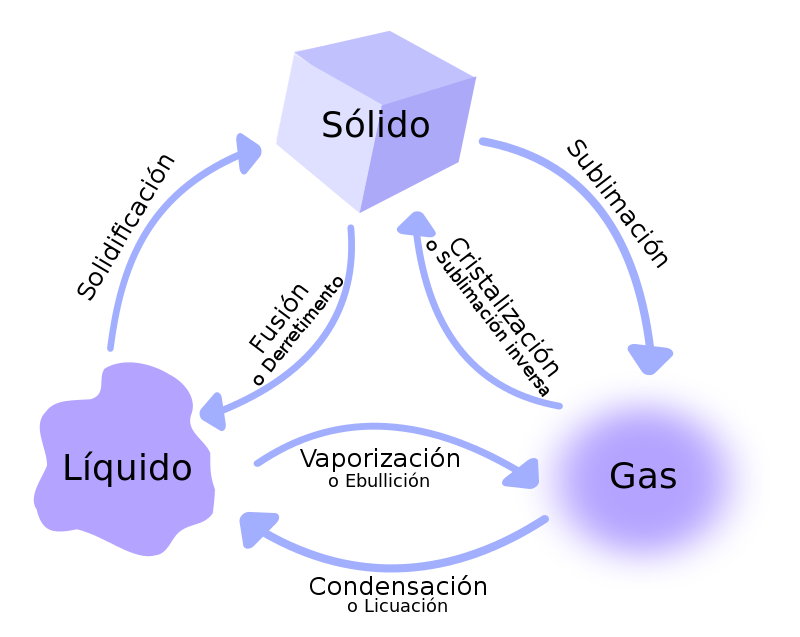
\includegraphics[scale=0.5]{imagenes/cambiosEstado} 
\end{center}


\begin{itemize}
\item La \textbf{vaporización} es el paso del estado líquido al gaseoso al calentarse.
\item La \textbf{condensación} es el paso del estado gaseoso al estado líquido al enfriarse.
\item La \textbf{fusión} es el paso del estado sólido al estado líquido al calentarse.
\item La \textbf{solidificación} es el paso del estado líquido al estado sólido al enfriarse.
\item La \textbf{sublimación} es el paso directo del estado sólido al estado gaseoso al calentarse.
\item La \textbf{sublimación inversa} es el paso directo del estado gaseoso al estado sólido al enfriarse.
\end{itemize}

Cada sustancia cambia de estado a una temperatura única y exacta, por ejemplo, el agua la vaporización ocurre cuando se calienta hasta los 100ºC, cuando se forman burbujas y se desprende mucho vapor. Esto es lo que denominamos ebullición. La temperatura de ebullición del agua es de 100\textdegree .

La condensación se produce cuando se enfría el vapor de agua por debajo de los 100\textdegree . Cuando esto ocurre, se van formando pequeñas gotas líquidas. Este efecto se puede observar en la tapa de una olla cuando se destapa. Al chocar el vapor con la superficie fría de la tapa se condensa.

La fusión del hielo se produce cuando este se calienta a temperaturas de 0\textdegree , y el hielo se transforma en agua líquida. La temperatura de fusión del agua es de 0\textdegree .

La solidificación tiene lugar cuando se enfría el agua por debajo de los 0\textdegree , y el líquido se congela, por ejemplo cuando se mete el agua en el congelador.

\section{Las mezclas}

\subsection{Mezclas homogéneas}
Las \textbf{mezclas homogéneas} son aquellas en las que \textbf{no podemos diferenciar} los componentes, también se llaman \textbf{disoluciones}. Son mezclas homogéneas el agua con sal, el agua con azúcar o el café.

 En la disoluciones tenemos un componente mayoritario que se llama \textbf{disolvente}, y uno o varios componentes en menor cantidad llamado \textbf{solutos}. Por ejemplo, en el agua del mar el disolvente será el agua y el soluto la sal.

\subsection{Mezclas heterogéneas}

Las \textbf{mezclas heterogéneas} son aquellas en las que \textbf{podemos diferenciar} los componentes, por ejemplo el granito o el agua con aceite.



\section{Separación de mezclas}

Se pueden separar los componentes de las mezclas por diferentes métódos, cada tipo de mezclas posee diferentes propiedades, no es lo mismo una mezcla de agua con sal que una mezcla de agua con arena. Es por esto por lo que es necesario conocer que tipo de mezcla tenemos entre manos para poder realizar la separación.

\subsection{Separación de mezclas heterogéneas}

Las mezclas heterogéneas se puede separar con algunos métodos sencillos. Algunos de estos son cotidianos como la filtración, la decantación y la separación magnética.

\subsubsection*{Filtración}

La filtración se emplea para separar sustancias sólidas que están en suspensión en un líquido. Para ello se hace pasar la mezcla a través de un filtro por el que el líquido pasa a través de los poros, mientras que el sólido permanece en el filtro. Este proceso se emplea en la cocina para separar la pulpa de la naranja del zumo.
\begin{center}
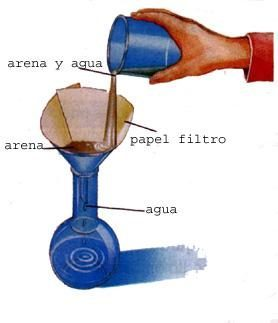
\includegraphics[scale=0.8]{imagenes/filtracion} 
\end{center}



\subsubsection*{Decantación}

La decantación se emplear para separar dos sustancias con densidades muy diferentes y que no se mezclan entre ellas y por tanto una flota sobre la otra. Para separarlas se emplea un instrumento llamado embudo de decantación, que tiene una válvula que al abrirla saca el componente que se encuentra en el fondo.
\begin{center}
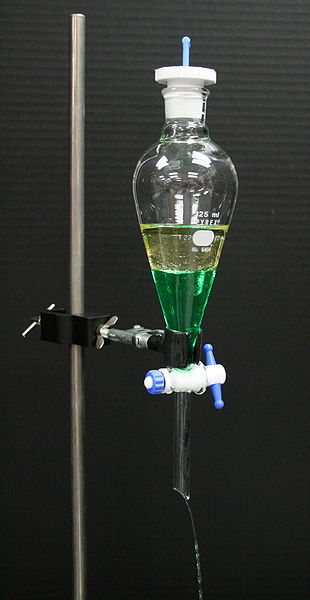
\includegraphics[scale=0.5]{imagenes/decantacion} 
\end{center}


\subsubsection*{Separación magnética}

La separación se emplea cuando tenemos una mezcla de metales en las que alguno son atraídos por un imán pero otros no. Este tipo de separación se emplea en las chatarrerías para separar el hierro de otros metales como el cobre o el aluminio.

\begin{center}
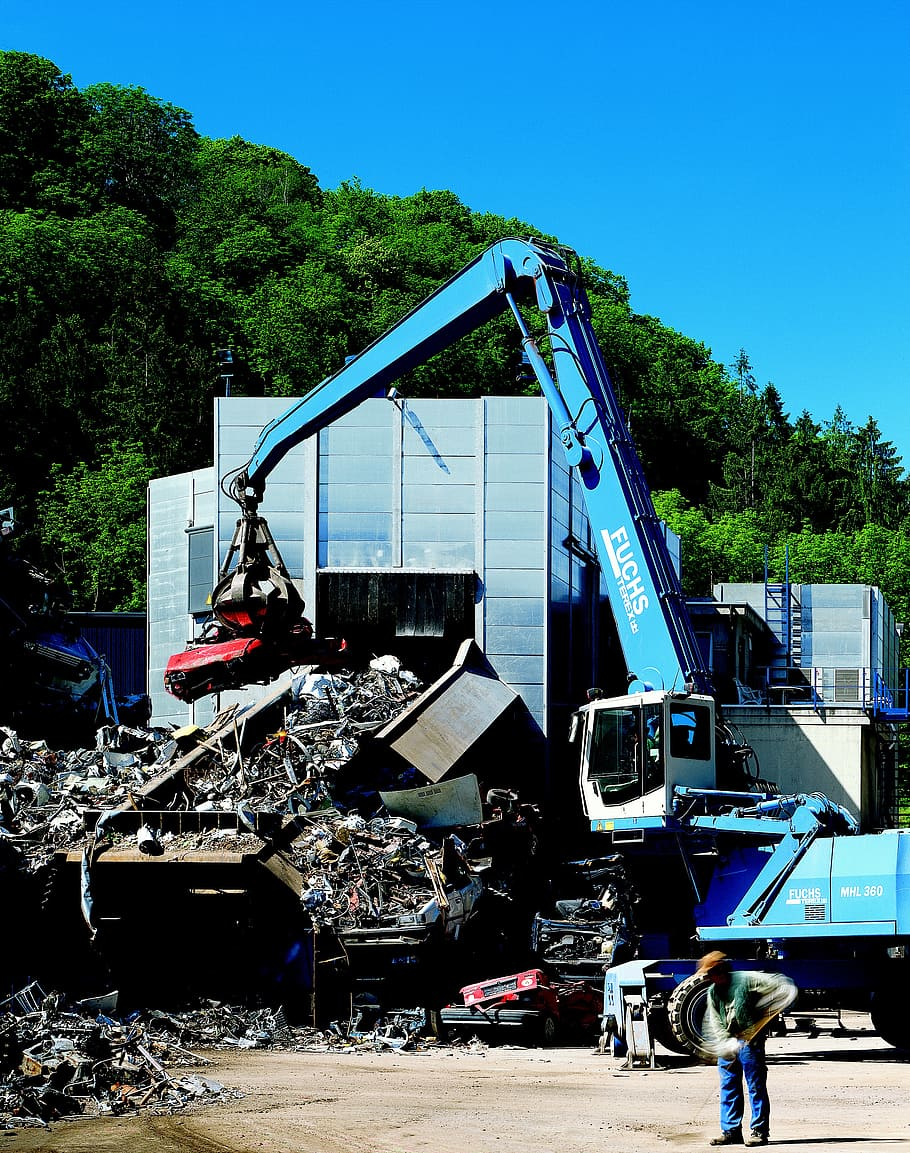
\includegraphics[scale=0.4]{imagenes/iman} 
\end{center}



\subsection{Separación de mezclas heterogéneas}

Para separar un sólido disuelto en un líquido no es posible usar técnicas como la filtración, por lo que necesitamos recurrir a otras como la evaporación del disolvente. Esto es lo que se realiza en las salinas, cerca del mar para conseguir la sal del agua del mar. 

\begin{center}
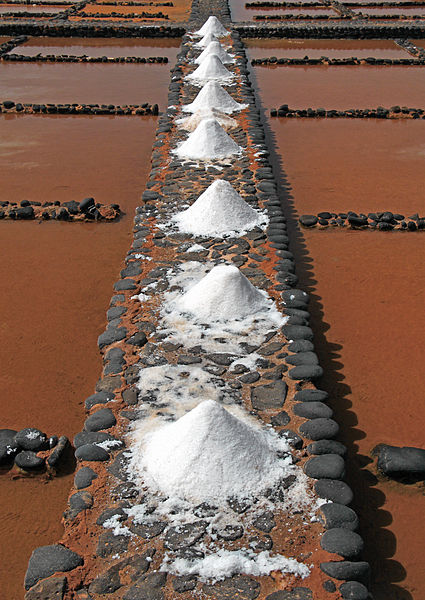
\includegraphics[scale=0.5]{imagenes/salinas} 
\end{center}


%\chapter{Cambios Físicos}
%\chapter{Cambios Químicos}
\chapter{La luz y el sonido}

\section{¿Qué es la luz?}

La luz es una forma de energía que nos permite ver todo lo que nos rodea como las formas y los colores de los objetos. Se propaga a una velocidad muy rápidca, casi instantánea para nuestros ojos, en el aire viaja a una velocidad de casi 300 000 km/s, es decir, en un solo segundo ha recorrido 300 000 km, o lo que es lo mismo, en un solo segudno daría la vuelta al mundo siete veces y media.

\section{¿Qué objetos transmite luz?}

Los objetos que emiten luz propia les llamamos \textbf{focos luminosos}, y los podemos diferenciar en:

\begin{itemize}
\item \textbf{Foco luminoso natural:} son aquellos que emiten luz propia de forma espontánea como el Sol. 

\item \textbf{Foco luminoso artificial:} son aquellos que emiten luz en determinadas condiciones, como una bombilla cuando se le suministra electricidad.

\end{itemize}


\section{¿Cómo se propaga la luz?}

En el aire, que es donde normalmente se propaga la luz, lo hace siempre en todas las direcciones y en línea recta. A cada una de estas líneas rectas les llamamos rayo luminoso.


\section{¿Cómo se comportan los objetos ante la luz?}

Los cuerpos que no emiten luz solo se puede ver cuando los iluminamos con un foco de luz. Estos cuerpos lo que hacen es reflejar parte de la luz que reciben y absorber la otra parte. Ante este hecho, podemos clasificar los cuerpos en \textbf{opacos}, \textbf{translúcidos} y \textbf{transparentes}.

\begin{itemize}
\item \textbf{Los cuerpos opacos:} son aquellos que no dejan pasar la luz. Cuando los rayos de luz llegan a un cuerpo opaco, estos rebotan.

\item \textbf{Los cuerpos translúcidos:} son aquellos que dejan pasar algo de luz, por lo que las imágenes que se perciben detrás de ellos son imágenes borrosas. Esto ocurre con algunos líquidos y vidrios como los de las mamparas de baño.


\item \textbf{Los cuerpos transparentes:} son aquellos que permiten el paso de toda la luz, por lo que los objetos de detrás de ellos se perciben de forma nítida. Por ejemplo, el vidrio de las ventanas, el agua clara o el aire.
\end{itemize}
%\chapter{Electricidad y magnetismo}
\chapter{El calor}

\section{¿Qué es el calor?}

El calor es una forma de energía que en nuestra vida cotidiana usamos para calentarnos, cocinar e incluso obtener electricidad. El calor siempre se transmite desde los objetos calientes a los fríos, es decir que cuando tenemos frío, realmente lo que pasa es que estamos perdiendo nuestro calor corporal; en cambio, cuando tenemos calor, lo que ocurre es que el objeto caliente nos pasa calor a nosotros. Esto es lo que ocurrire en verano cuando nos ponemos a tomar el Sol.

La cantidad de calor que posee un cuerpo es lo que llamamos temperatura, y para medirla usamos un termómetro.

\section{¿Cómo se transmite el calor?}

Ya hemos visto que el calor pasa siempre del foco caliente al foco frío, pero cómo ocurre esto. Pues la trasmisión de calor puede ocurrir mediante tres mecanismos diferentes: \textbf{conducción}, \textbf{convección} y \textbf{radiación}.

\subsection{Conducción}

En los objetos sólidos, el calor se transmite por coducción. Esto es lo que ocurre cuando sujetas un objeto metálico por un extremo y pones el otro extremo al fuego. Al final, aunque la llama no toca el extremo por el que lo sujetas, acabarás quemándote, ya que el calor se ha ido transmitiendo. Pero este fenómeno no ocurre con todos los objetos, si en lugar de un alambre cogemos un palo de madera, al ponerlo al fuego el extremo por el que lo sujetas no se calentará. ¡Ojo, aunque no se caliente, si se puede quemar, porque es madera!

A los objetos como  el alambre que si transmiten el calor les llamamos \textbf{conductores}, todos los metales son conductores. Mientras que a los objetos que no transmite en calor los llamamos \textbf{aislantes}, la madera, el plástico o el poliestireno (el corcho blanco de embalar), son buenos aislantes del calor.

\subsection{Convección}

Los objetos en estado líquido o gaseosos, pueden transmitir el calor por convección. Por ejemplo, al calentar agua en una olla la parte de abajo se calienta y sube, mientras que la superficie con agua fría baja, producciendo una circulación de agua que llamamos corrientes de convección. Esto mismo también ocurre en la atmósfera, produciendo fenómenos como el viento.


\subsection{Radiación}

En cambio, cuando no existe un contacto directo con la fuente de calor, también se puede transmitir calor por radiación. De esta forma el Sol calienta nuestro planeta. Es el mecanismo más débil para transmitir calor, ya que al no existir contacto se pierde efectividad.



\section{¿Qué efectos produce el calor?}

Seguro que alguna vez has intentado abrir una puerta de acero en verano y se atasca, cosa que no ocurría con esta misma puerta en invierno. Esto se debe a que el calor al modificar la temperatura de los objetos, también es capaz de variar su tamaño. Es lo que llamamos \textbf{dilatación} y \textbf{contracción}.

\subsection{La dilatación}

La dilatación consiste en el aumento de tamaño de un objeto al aumentar su temperatura, es decir, al calentarse. Esto ocurre en los raíles de las vías del tren así como en los puentes, por esto cuando se monta un puente o una vía de tren, se deja un hueco entre pieza y pieza. 

\subsection{La contracción}

En el otro lado, la contracción es la disminución de tamaño de un objeto debido a la disminución de su temperatura, es decir, cuando se enfría. 



\section*{Actividades}

\begin{enumerate}
\item{Completa las siguientes frase:
El \hrule{5cm} se transmite de los cuerpos calientes a los cuerpos fríos. 
La cantidad de \hrule{5cm} que tiene un cuerpo es la \hrule{5cm}.
La \hrule{5cm} tiene lugar cuando un cuerpo aumenta de tamaño, debido a un aumento de temperatura.
La \hrule{5cm} es el efecto contrario y se produce cuando el cuerpo se enfría.}

\item{Dí que forma de transmisión de calor corresponde a cada dibujo.}

%Poner dibujos.

\item{Observa la image y explica por qué se deja estos espacios en los puentes.}




\end{enumerate}
\chapter{La energía}
%\chapter{Las máquinas}

\nocite{*}
\bibliographystyle{plain}
\bibliography{referencias}


\end{document}
